\begin{textblock*}{3cm}(0cm,-1cm) % {block width} (coords)
    \begin{tikzpicture}
        \fill[ERDCRed] (0,0) rectangle (3,29.1); % Fill for the sidebar
        \draw[white, thick] (0.1,0.1) rectangle (2.9,29.11); % White border for aesthetic
    \end{tikzpicture}
\end{textblock*}

% Add vertical text for the book title
\begin{textblock*}{40cm}(1cm,10cm) % Adjust the width and position of the text block to accommodate larger text
    \rotatebox{90}{
        \fontsize{40}{48}\selectfont % Adjusted for better fit
        \textbf{\color{white}Part Two} % Change text here
    }
\end{textblock*}
\newgeometry{left=5.81cm, top=1in, bmargin=1in, right=1in}
\begin{center}
\section{Distributed Cognition \hspace{0.1cm} \color{white}2}
\end{center}
\subsection{Unit of Analysis}
The unit of analysis in this case is the socio-technical system comprising the noise management system in the library environment. This includes the technological components, such as the display, microphone, networking, map of the library, anonymous messaging system, volume meter, decibel count, auditory cues, and desk vibrations. There are also the human elements, such as the library users and librarians, not only as individuals, but also as groups of people. Environmental factors, such as the design of the library space, the placement of the devices and desks, and overall accoustics can impact the effectivness os the system, and users' perceptions. This leads us to the cognitive processes involved, such as the afformentioned perception of the device, social communication between users through the devices, memory and learning from the system to help users learn and internalize acceptable noise levels, the live decision making processes due to the real-time feedback of the device based on their actions, the feedback loops that may occur as the device influences users' actions, and the formation of loops between users' due to the possibility of a new social norm emerging. Finally, it may be important to consider other external factors, such as the policies of the library and it's location.
\begin{figure}[h]
    \centering
    \frame{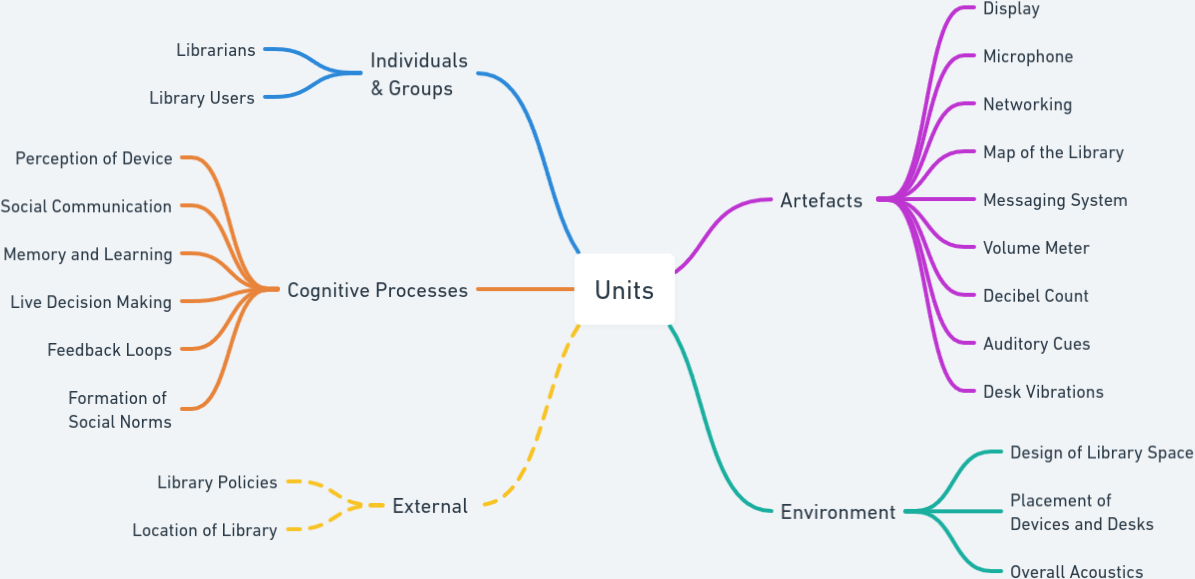
\includegraphics[width=1\textwidth]{images/unit}}
    \caption{Unit of Analysis}
\end{figure}

\restoregeometry


\newgeometry{left=3.81cm, top=1in, bmargin=0.9in, right=1in}

\begin{textblock*}{3cm}(0cm,-1cm) % {block width} (coords)
    \begin{tikzpicture}
        \fill[ERDCRed] (0,0) rectangle (1,29.1); % Fill for the sidebar
        \draw[white, thick] (0.1,0.1) rectangle (0.9,29.11); % White border for aesthetic
    \end{tikzpicture}
\end{textblock*}

\newpage
\subsection{Memory Represenatations}

One aspect of memory is the individuals users recognition and recall of the color-coded desks, volume metre, and decibel count. These visual cues help users remember the appropriate noise levels for different areas of the libraries. This encourages a social conformance, where users avoid being the odd one out. Over time users may begin to assoiate specific shades of colors with what the appropriate noise levels are, without needing to compare and refer to the colors of the other desks on the display. Gentle auditory and tactle feedback serve as an immediate reminder for users to lower their volume, helping to interrupt and modify loud behavour, and possibly culling the formation of bad habits. This real-time feedback from multiple sources helps uses learn the corrolation between their percieved loudness and the actual noise level. These signals aid users in adjusting their behaviour based on past experiences with the device, reinforcing quieter behavior.

It is likely that the impact on collective memory would be far more significant. By encouraging social conformity by making noise levels visible and subject to community policing, the system is likely to cause cultural shift. If these changes were to occur, they would become a part of the collective memory of the library, altering the experience for new and returning visitors. 
%TC:ignore
\bgroup
\def\arraystretch{1.22}%
\begin{longtable}{
    ||  
        >{\centering\arraybackslash}m{0.25\textwidth} 
    |
        >{\raggedright\arraybackslash}m{0.68\textwidth}
    ||} 
    \hline
\multicolumn{2}{||c||}{\textbf{Internal Human Memory}} \\
 \hline
Short-term Memory               & Noticing and reacting to the live device outputs.               \\
Long-term Memory                & Recognizing and recalling color-coded desks, associating colors with appropriate noise levels. Avoiding creating noise by remembering the visual and haptic cues that would occur if volume is too high.                                  \\
Procedural Memory               & Learning and internalizing the process of adjusting volume based on feedback from the system.       \\
\hline 
\hline
\multicolumn{2}{||c||}{\textbf{Internal System Memory}} \\
 \hline
Persistent Storage              & Storing the map of the library, messages, and historical noise levels to allow comparisons and data analysis.                             \\
Operational Memory              & Processing real-time noise levels, updating the display, and sending messages or feedback.                                 \\
 \hline
 \hline
\multicolumn{2}{||c||}{\textbf{Collective Memory}} \\
 \hline
Social Norms                         & Forming new social norms on acceptable noise levels. \\
 \hline
 \hline
  \multicolumn{2}{||c||}{\textbf{External System Memory}} \\
 \hline
Physical Interface              & Display with a top-down view of the library with color-coded desks based on their volume, standard volume meter, decibel count, messaging app.                                      \\
Feedback Mechanisms             & Anonymous messaging system, auditory cues, desk vibrations.  \\
 \hline
 \caption{Table of Categorised Memory Representations}
\end{longtable}
\egroup
%TC:endignore
\begin{textblock*}{3cm}(0cm,-1cm) % {block width} (coords)
    \begin{tikzpicture}
        \fill[ERDCRed] (0,0) rectangle (1,29.1); % Fill for the sidebar
        \draw[white, thick] (0.1,0.1) rectangle (0.9,29.11); % White border for aesthetic
    \end{tikzpicture}
\end{textblock*}

\newpage
\subsection{Information Flow}
\vspace{-0.5cm}
\begin{figure}[h]
    \centering
    \caption{Basic Information Flow}
    \vspace{0.2cm}
    \subfigure{\frame{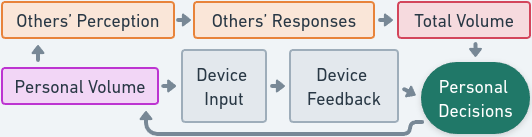
\includegraphics[width=0.82\textwidth]{images/small-flow}}}
    \subfigure{\frame{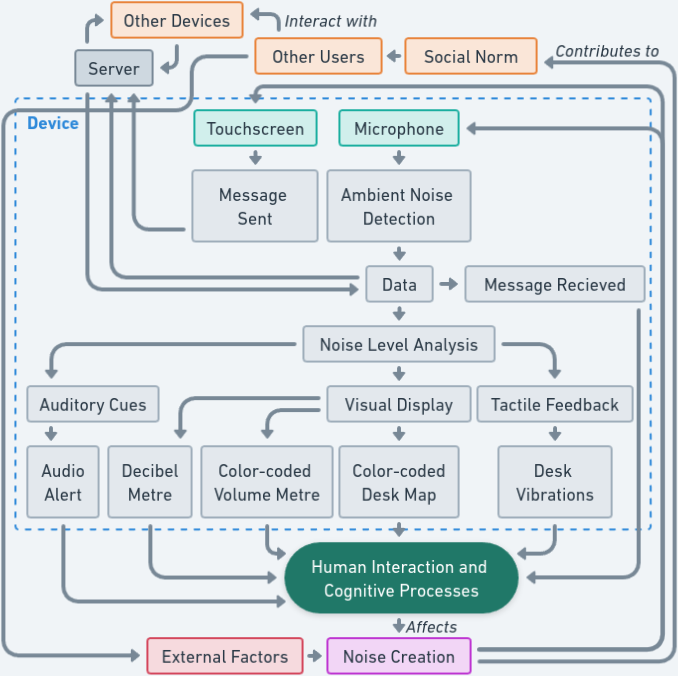
\includegraphics[width=0.82\textwidth]{images/big-flow}}}
    \caption{Detailed Information Flow}
\end{figure}
\vspace{-0.25cm}
\noindent
These figures show how the device can interrupt the typical feedback loop of noise increasing when people have to speak louder than those around them to be heard. With a device that provides immediate feedback, the user is likely to lower their voice, which, in turn, is likely to encourage others to follow suit.

\begin{textblock*}{3cm}(0cm,-1cm) % {block width} (coords)
    \begin{tikzpicture}
        \fill[ERDCRed] (0,0) rectangle (1,29.1); % Fill for the sidebar
        \draw[white, thick] (0.1,0.1) rectangle (0.9,29.11); % White border for aesthetic
    \end{tikzpicture}
\end{textblock*}


\newpage
\subsection{Computation and Processing}
The information flow in figure 4 demostrates the technological requirements in the device to allow computation and processing. The device primarily deals with real-time audio analysis, likely involving Fourier transforms or similar algorithms to break down audio signals into decibel levels. These devices continuously monitor the ambient noise in different sections of the library. Sound levels must be captured accurately, filtering background noise, and converting acoustic signals into digital decibel readings. Advanced signal processing techniques may be required to ensure accuracy and minimize false alarms. Graphical user interfaces and mapping software that present a top-down view of the library require responsive touchscreens. Real-time data processing to update the map based on noise levels detected by microphones. Color coding is applied to represent different noise levels, requiring algorithms to translate decibel readings into color signals on the display. The infrastructure to support anonymous messaging between desks must handle data transmission securely and efficiently. This includes server-side processing to manage messages, client-side processing to display messages, and network protocols to ensure timely and confidential communication. Generating auditory cues and desk vibrartions requires a controller that can interpret noise level inputs and trigger appropriate feedback mechanisms. The vibration motors and audio outputs must be calibrated to deliver noticeable yet discreet signals. The system must manage and process feedback loops between the users' behavior and the system's outputs. For example, if a desk continues to be noisy despite feedback, the system might escalate the warnings or notify library staff.

Processing also takes place on the human side. The system's effectiveness is partially dependent on how users perceive and react to the feedback. While the device can act on multiple difference senses, it still requires users to be aware enough to act on. Users must also learn to associate colors, sounds and vibrations with appropriate noise levels, requiring a certain level of cognitive processing.

\subsection{Problems}
The past few sections offered a detailed insight into how the Distributed Cognition analysis supports the design. However, it is also important to consider the cognitive load this system will have on users, as well as possible shortcomings within the analysis.

Constant vigilance can be mentally exhausting, particularly over long periods. It might also lead to anxiety or stress over activating the alerts. Users are likely to see these devices as intrusive and a waste of space, causing a poor experience design. Sounds, vibrations, and dynamic displays may be more distracting to humans than background conversations. Lastly, it is difficult for users to know whether the devices are listening in on their conversations, and may lead to privacy concerns.

This Distributed Cognition analysis does not provide us with any empirical measurments. It is difficult to conlude whether the microphone inputs and algorithms would be accurate enough to correctly altert users. A purely theoretical model cannot be a basis for implementation until real world tests are carried out.

%TC:ignore
\begin{textblock*}{3cm}(0cm,-1cm) % {block width} (coords)
    \begin{tikzpicture}
        \fill[ERDCRed] (0,0) rectangle (1,29.1); % Fill for the sidebar
        \draw[white, thick] (0.1,0.1) rectangle (0.9,29.11); % White border for aesthetic
    \end{tikzpicture}
\end{textblock*}
%TC:endignore
\restoregeometry